\section{Computational Steering Using Sparse Grids}

% The application which we ported on heterogeneous systems is

% This numerical technique allows us to cope with curse of dimensionality. 
% Fig. \ref{fig:big_picture} depicts an example of 5d data, i.e. velocity field,
% obtained from simulating the lid driven cavity for different  Reynolds numbers (Re).
% The lid driven cavity is a classical problem in Computational Fluid Dynamics (CFD). 
% The velocity of cavity's upper wall can also be transformed into a parameter,
% making this a 6d problem.

Managing the data coming from functions with high number of dimensions can pose
serious challenges. Therefore, we compress the data using the sparse grid
technique in order to reduce its size and we decompress it afterwards for
real-time visualization. Compressing a general function represented on a full
grid is done by selecting only the function values at grid points also contained
in a sparse grid. This is reduced to computing the hierarchical coefficients,
process called hierarchization. Decompression (or interpolation) refers to
evaluating the function anywhere inside the domain by summing up the
contributions of the basis functions averaged by their hierarchical
coefficients. This technique also enables us to interpolate at points for which
we do not have values from simulation. Hence, it can provide hints on the
simulation outside the initial data.

Our application is the visualization of compressed, high-dimensional data
resulting from simulations \cite{butnaru2011}. Decompression is in our case a
form of interpolation based on the sparse grid technique described in
\cite{bungartz2004}. To allow a fluent interaction with data, interpolation has
to run as fast as possible. This is equivalent to ensuring that no processor in
a heterogeneous system is idle at any moment of time and that each processor is
used at its full potential.



% This technique also enables us to interpolate at points for which we do not
% have values from simulation.
% This can be seen as a non-expensive way to obtain hints about the behavior of
% the simulation outside the initial data without running the simulation.

% The sparse grid technique is a numerical technique for representing
% high-dimensional functions. Sparse grid interpolation is the essential
% component of our visualization application. Consequently, to allow a fluent
% interaction with data, interpolation has to run as fast as possible. This is
% equivalent to ensuring that no processor in a heterogeneous system is idle at
% any moment of time and that each processor is used at its full potential.

% \begin{figure}[bp]
%   \centering
%   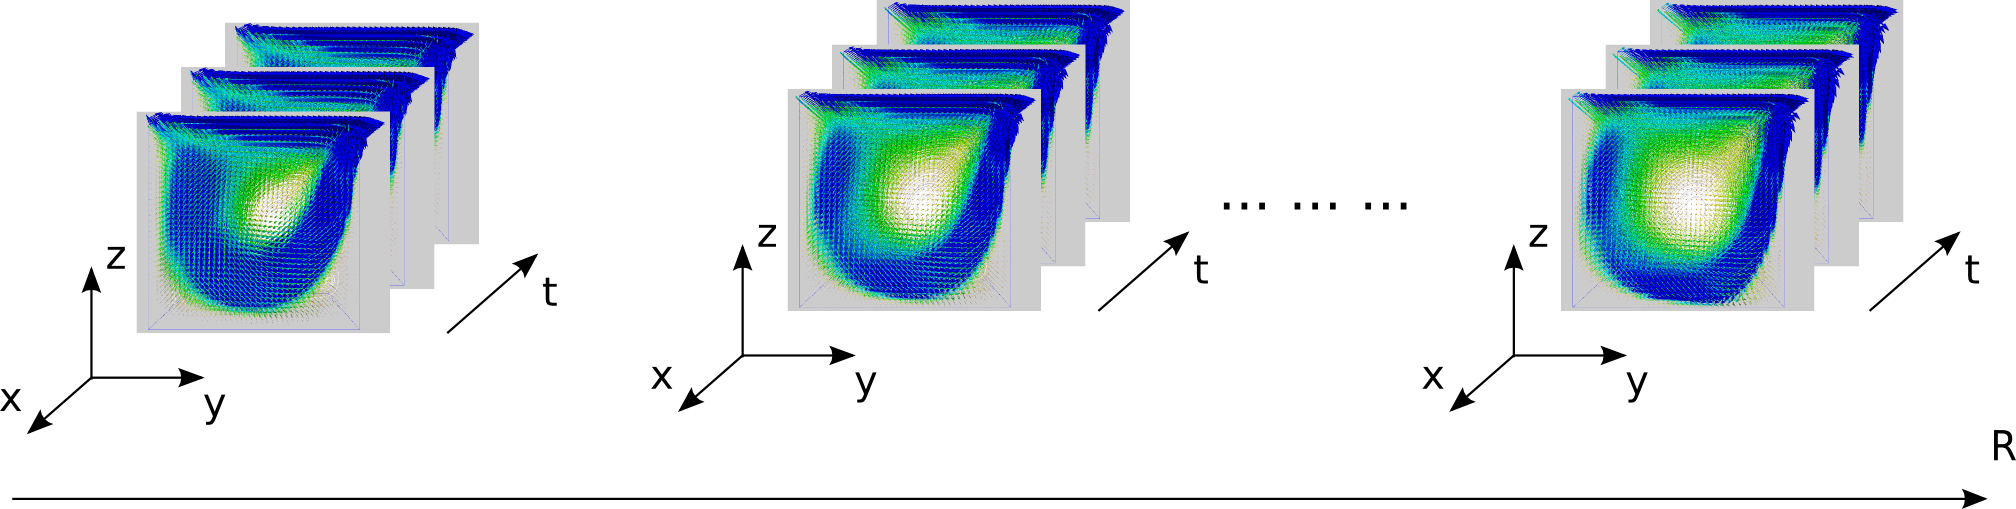
\includegraphics[width=0.85\textwidth]{big_picture}
%   \caption{5d (x, y, z, t, Re) data from a CFD simulation.}
%   \label{fig:big_picture}
% \end{figure}

Sparse grid interpolation has 5 input parameters: the number of dimensions (D),
the refinement level (L), the number of interpolations (N), the precision (P)
(single or double precision), and the adaptivity (A) (adaptive or regular). In
this paper we concentrate on the first 3, these being the most important as they
can take a wide range of values. 

% Fig.~\ref{fig:bigger_sparse_decomposed} (left) shows that a sparse grid can be
% represented as a sequence of regular grids \cite{murarasu2011}.
% This is the central idea of the bijection based data structure from
% \cite{murarasu2011} which features minimal memory consumption.
% Using this storage scheme, we can explain the interpolation and the impact of
% the inputs on performance. Interpolating
% (Fig.~\ref{fig:bigger_sparse_decomposed} (right)) at a given D-dimensional point
% means traversing the set of regular grids and computing the contribution of each
% regular grid on the result. For each regular grid a D-linear basis function
% (\Otime{D}) is built and evaluated at the point. Interpolating at one point uses
% exactly one value from each regular grid for scaling the basis function.
% Using this knowledge, we can now look at the influence of the inputs on performance. 
% All of these parameters influence to some extent the performance behavior of interpolation, especially on the GPU.

D increases the computational intensity, i.e. the ratio between the on-chip
computation time and off-chip communication time. On GPU, a large D causes an
increased consumption of shared memory per thread reducing the benefits of
multithreading. A large L decreases the computational intensity since the size
of the regular grids increases exponentially, i.e. from $2^0$ to $2^{L-1}$. 

As only one regular grid value is used per interpolation, only a small
percentage of the compressed data transferred over PCIe to the GPU is actually
used for computation. N is proportional to the computational intensity, i.e the
more interpolations we perform, the more worthwhile is the data transfer over
PCIe.

The dimensional adaptivity parameter gives the possibility of reducing the
computational effort when using functions where not all input variables carry
equal weight. Therefore, instead of storing all regular grids, we can exclude
some of them when the information on those dimensions is not critical.

% \begin{figure}[tbp]
%   \centering
%   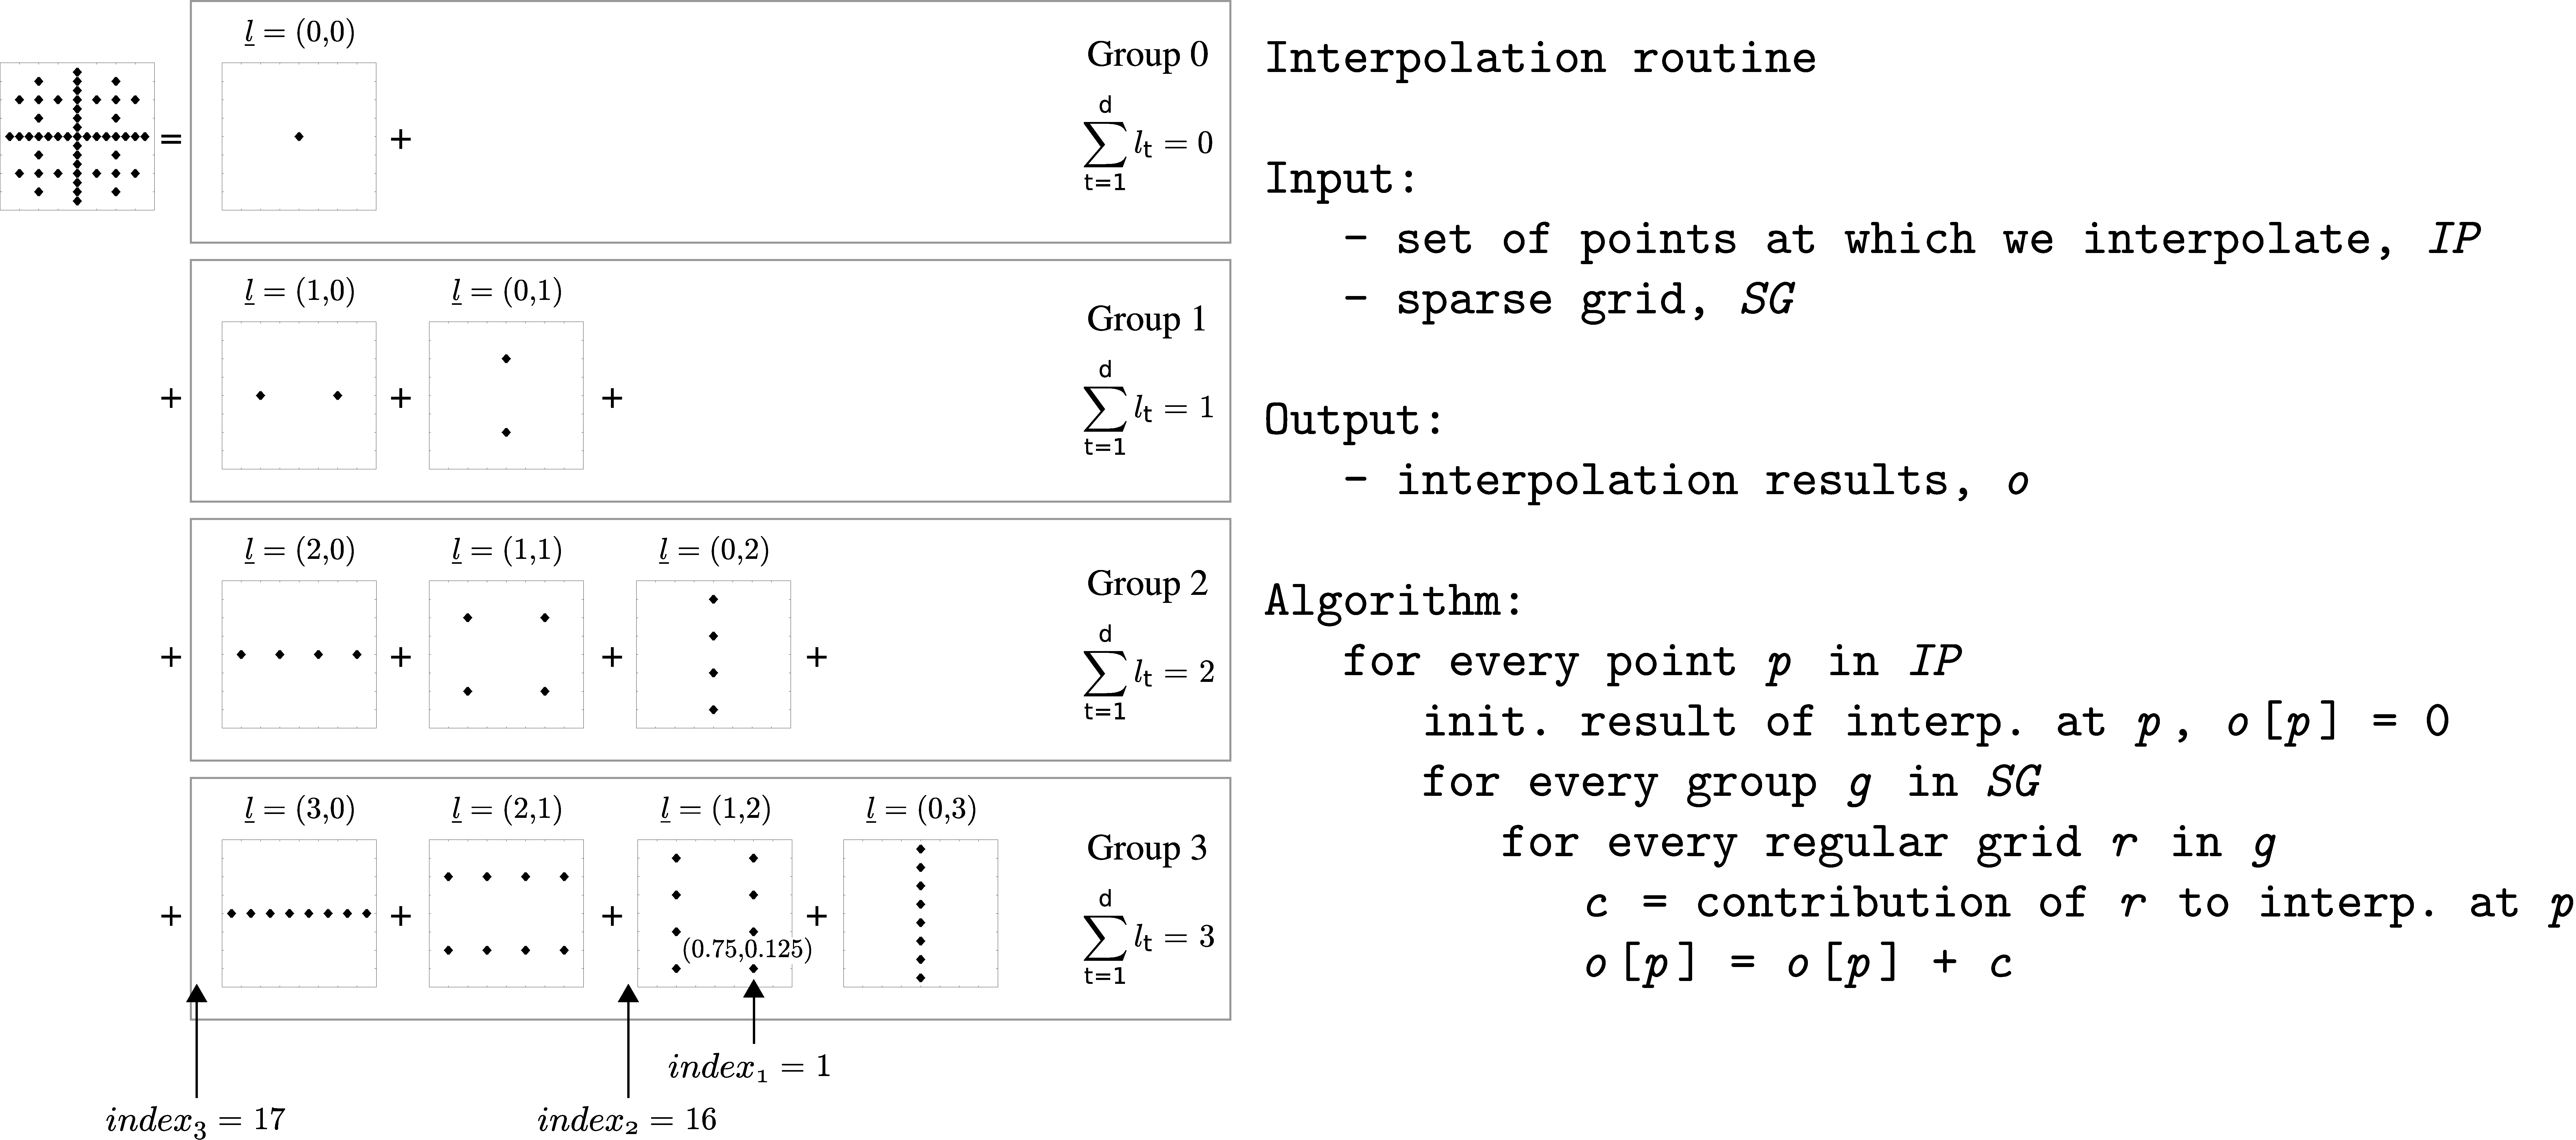
\includegraphics[width=\textwidth]{bigger_sparse_decomposed_new}
%   \caption{Left: 2d sparse grid decomposed as a sequence of regular grids. Group~l (l = $0 \dots 3$) contains $C_{D+l-1}^l$ regular grids of size $2^l$. D expands the groups horizontally while L expands them vertically. Right: simplified interpolation.}
%   \label{fig:bigger_sparse_decomposed}
% \end{figure}

Our versions of interpolation are based on the iterative algorithm from \cite{murarasu2011}. 
% The most important characteristic of this algorithm is that it is vectorizable.
The CPU version is optimized for best use of caches and vector units. Our GPU
implementation includes the following optimizations: coalesced memory accesses,
use of shared memory, no bank conflicts, etc. Having these two versions of
interpolation, we combine them so that all the processors in a heterogeneous
system simultaneously work on interpolation. In general, on the systems where
we measured the performance of interpolation, the GPU was faster than the CPU.
But, since our goal is performance portability, it makes sense to consider the
situation in which the GPU is not faster than the multi-core CPUs available in
the system. This can be the case for instance with Intel's Sandy Bridge
processors which have a SIMD unit~\cite{avx} (256~bit AVX) twice as wide as the
previous generation, Nehalem (128~bit SSE). The parallelization of sparse grid
interpolation is based on distributing the points for interpolation among
threads.
% Note that typically, we interpolate at minimum $10^5$ points. 